\documentclass[AutoFakeBold]{ctexart}

% 基础宏包

\usepackage[utf8]{inputenc}
\usepackage[T1]{fontenc}
\usepackage[english]{babel}

% 数学宏包
\usepackage{amsmath}
\usepackage{amssymb}
\usepackage{amsthm}
\usepackage{siunitx}
% 图形和表格
\usepackage{graphicx}
\usepackage{subcaption}
\usepackage{float}
\usepackage{booktabs}

% 页面布局
\usepackage[
a4paper,
margin=2.54cm
]{geometry}
\usepackage{fancyhdr}
\usepackage{titlesec}

% 参考文献和引用
\usepackage{natbib}
\usepackage{hyperref}
% 使用 hypersetup 设置 hyperref 的选项
\hypersetup{
	colorlinks=true,
	linkcolor=blue,
	citecolor=red,
	urlcolor=magenta
}

% 颜色和绘图
\usepackage{xcolor}
\usepackage{tikz}

% 代码和算法
\usepackage{listings}
\usepackage{xcolor}
\lstset{
	numbers=left, 
	numberstyle= \tiny, 
	keywordstyle= \color{ blue!70},
	commentstyle= \color{red!50!green!50!blue!50}, 
	frame=shadowbox, % 阴影效果
	rulesepcolor= \color{ red!20!green!20!blue!20} ,
	escapeinside=``, % 英文分号中可写入中文
	xleftmargin=2em,xrightmargin=2em, aboveskip=1em,
	framexleftmargin=2em
} 

\usepackage{algorithm}
\usepackage{algpseudocode}

% 其他常用宏包
\usepackage{enumitem}
\usepackage{siunitx}
\usepackage{blindtext}
\usepackage{verbatim}
% 自定义页面布局
\geometry{margin=2.5cm,a4paper}
\pagestyle{fancy}
\fancyhf{}
\fancyfoot[C]{\thepage}

% 自定义标题格式
\titleformat{\section}{\large\bfseries}{\thesection}{1em}{}
	
% 文档开始
\begin{document}
	
	% 摘要部分独占一页
	
	\pagenumbering{arabic}
	\setcounter{page}{2}
	%\thispagestyle{plain}
	% 论文正文部分
	\section{问题重述}
	\subsection{问题背景}
	\songti\zihao{-4}砷是一种有毒的重金属元素,在水体中主要以砷离子 [As(V)] 和洛克沙胂(ROX)两种形式存在。目前,全球水体砷污染问题严重,长期饮用含砷的水会导致多种严重的健康问题,包括皮肤病、癌症以及心血管疾病,极大地危害了人类的健康。因此,如何有效地去除水体中的砷成为亟待解决的问题。
	
	\songti\zihao{-4}探索改性生物碳在高效吸附有机无机砷方面的工艺条件,对于改善水体砷污染问题具有重要的意义和价值。通过数学建模,可以系统地研究上述因素对吸附过程的影响,优化吸附条件,提高砷去除效率,从而为水体砷污染的实际处理提供科学依据和技术支持。
	\subsection{问题要求}
	\songti\zihao{-4}附件1中所给出的是吸附剂用量、温度及pH的变化对ROX和As(V)的去与吸附率相关实验的情况。为探索改性生物碳高效吸附有机无机砷的工艺条件以改善水体砷污染的问题,现需结合所给实验信息建立数学模型并分析以下问题:
	
	\songti\zihao{-4}问题一:依据附件1中所给实验数据,用控制变量法分别研究反应温度、溶液pH及吸附剂的用量对As(V)和ROX去除率的影响,探讨其是否具有一定的相互关系。
	
	\songti\zihao{-4}问题二:通过对附件1中所给实验数据来研究所给的三种影响条件在何种情况下可以使As(V)和ROX的总吸附量最大。

	\songti\zihao{-4}问题三:基于现有实验情况下如何设计五组新的实验来进一步更好地研究As(V)和ROX的吸附情况。
	
	

	
	\section{问题分析}
	\songti\zihao{-4}改性生物碳对水中洛克沙胂和砷离子的吸附问题提供了关于ROX去除率,As(V)去除率ROX吸附量,As(V)吸附量四组有关pH,温度,吸附剂用量的数据,题目要求以此来选择最适的反应温度,溶液pH,吸附剂用量,并要求设计添加五次实验.由于给与的数据并不全面,在实验中具有诸多不确定性,只能分析出基本的自变量对吸附率的走向,因此需要增加在由分析出的最高值附近数据的实验,保证实验的可靠性与准确性。
	\subsection{问题一的分析}
	\songti\zihao{-4}问题一要求在其他反应条件一致的情况下,探讨反应温度,pH,吸附剂用量对去除率的影响
	建立起其中的数学模型,筛选出最为合适的变量范围,首先,对附件1的数据进行\textbf{预处理},确保预处理后的数据不存在错误,接着针对预处理后的数据,进行探索性的数据分析,观察各变量对于去除率的影响,建立起\textbf{综合多变量模型}。
	\subsection{问题二的分析}
	\songti\zihao{-4}问题二为考虑基于最大总吸附量的各变量大小的裁定。
	问题二要求求出最大总吸附量下,温度,pH,吸附剂用量数据的取值,基于问题一的实验数据处理方法,我们可以得出影响总吸附量的变量变化趋势,通过对已有吸附模型的优化,以及数据的处理与筛查,建立起适合题目的吸附模型,从而求解各变量的取值。
	\subsection{问题三的分析}
	\songti\zihao{-4}问题三要求增设5个实验并给出理由,因此在本题解答中针对模型的中心点重复以及边界等问题,我们给出了\textbf{中心点重复实验、边界探索性实验、敏感性分析实验、验证实验、环境因素识别实验}等5个实验对上述模型及相关数据进行检验与分析,以此确保实验模型的稳定性及健壮性。
		
	\section{数据预处理}
	1.数据整合
	
	观察题目中附件信息,可以发现它负有一定的规律性,同时琐碎冗杂,是典型的实验数据,对其每一项结果都进行数据筛查有利于保证后续实验数据的纯洁性与有效性
	
	2.处理方法
	
	对于需要对多数列进行检测的数据,本文选择使用\textbf{四分位数方法}\cite{张云华2009统计学中四分位数的计算}来识别异常值,寻找每个数值型列的潜在异常值,这使得无论数据是否符合正态分布,都可以被有效地处理,也可以尽可能多的保留实验的有效数据
	
	3.异常数据处理
	
	将实验数据进行IQR方法进行处理,去除明显高于其他周边数据的异常点,经过Python相关代码处理后,删去15条实验记录,如表1[\ref{tab:data}]所示.
	\begin{table}[H]
		\centering
		\begin{tabular}{|c|c|c|c|c|c|c|c|}
			\hline
			序号 & pH & 吸附剂用量 &温度& ROX吸附量 & As(V)吸附量 & ROX 吸附率 & As(V)吸附率 \\
			\hline
			0  & 3 & 0.2 & 15 & 40.38 & 4.93 & 77.56 & 92.49 \\\hline
			1  & 3 & 0.2 & 25 & 39.98 & 4.90 & 77.03 & 93.12 \\\hline
			2  & 3 & 0.2 & 30 & 40.17 & 5.00 & 75.65 & 93.47 \\\hline
			3  & 3 & 0.2 & 35 & 39.00 & 5.13 & 75.90 & 94.18 \\\hline
			4  & 3 & 0.2 & 45 & 34.52 & 4.90 & 80.60 & 94.03 \\\hline
			25 & 5 & 0.2 & 15 & 40.10 & 5.10 & 77.23 & 91.57 \\\hline
			26 & 5 & 0.2 & 25 & 39.70 & 4.92 & 76.82 & 92.19 \\\hline
			27 & 5 & 0.2 & 30 & 39.89 & 4.78 & 74.89 & 92.54 \\\hline
			28 & 5 & 0.2 & 35 & 38.73 & 4.93 & 75.65 & 93.24 \\\hline
			29 & 5 & 0.2 & 45 & 34.28 & 4.85 & 79.53 & 93.09 \\\hline
			50 & 6 & 0.2 & 15 & 39.86 & 4.90 & 77.05 & 89.44 \\\hline
			51 & 6 & 0.2 & 25 & 39.46 & 5.02 & 76.40 & 90.05 \\\hline
			52 & 6 & 0.2 & 30 & 39.65 & 4.93 & 74.38 & 90.39 \\\hline
			53 & 6 & 0.2 & 35 & 38.49 & 4.95 & 74.79 & 91.07 \\\hline
			54 & 6 & 0.2 & 45 & 34.07 & 4.98 & 78.89 & 90.93 \\\hline
			79 & 7 & 0.2 & 45 & 14.47 & 5.10 & 35.90 & 93.95 \\
			\hline
		\end{tabular}
		\caption{无关数据表}
		\label{tab:data}
	\end{table}
	\section{模型假设}
	
		
		1.实验条件除pH,温度,吸附剂用量外,其余条件保持相同
		
		2.实验中的ROX与As(V)初始浓度未达到饱和
		
		3.改性生物碳在吸附过程中吸附力稳定,多层结构不发生显著变化
	
	
	

	
	

	
	\section{符号说明}

	\begin{table}[H]
		\centering
		\begin{tabular}{ccc}
			\toprule
			符号 & &含义 \\
			\midrule
			$C_e$ & & 平衡浓度 \\
			$Q_e$ & & 吸附量 \\
			$R$ & & 吸附率 \\
			$m$ & & 吸附剂用量 \\
			\bottomrule
		\end{tabular}
		\caption{模型公式所用的符号解释表}
		\label{tab:example}
	\end{table}
	
	
	\section{模型的建立与求解}
	
	\subsection{问题一}
	

	
	\begin{table}[H]
		\centering
		\begin{tabular}[H]{c}
			\toprule
			$Y_1$=127.885+16.365$X_1$-0.009$X_2$-10.974$X_3$ \\
			$Y_2$=96.754-1.139$X_1$+0.045$X_2$-0.462$X_3$\\
			\midrule
		\end{tabular}\\
		\begin{tabular}[H]{cccccccc}
			$X_1$  &   &   &  && &&  \qquad  吸附剂用量g/L  \\
			$X_2$ &   &   &  &&  & & \qquad 温度(摄氏度)   \\
			$X_3$ &   &   &  && &  & \qquad pH   \\
			$Y_1$ &  &   &  & && &  \qquad ROX去除率(\%)   \\
			$Y_2$  & & &  &&  & & \quad As(V)去除率(\%)  \\
			\bottomrule
			\midrule
		\end{tabular}\\
			\caption{去除率的算法及式中参数的含义}
		\label{tab:example}
	\end{table}
	
	\songti\zihao{-4}对于模型1ROX去除率,温度显著性较强,是主要的影响因素,由多元线性模型的系数可得出各变量对于去除率的影响。即pH对去除率有正向作用,而温度,吸附剂用量对于去除率起到负向作用。
	
	\songti\zihao{-4}对于针对As(V)去除率的模型二,显著性较强的是吸附剂用量,以99\%的显著性占据主要因素,对于该模型,不难看出吸附剂用量与pH起到负向作用,而温度在数据范围中与去除率呈现正相关。
	

	
	
	\begin{figure}[H]
		\centering
		\begin{minipage}{0.45\textwidth}
			\centering
			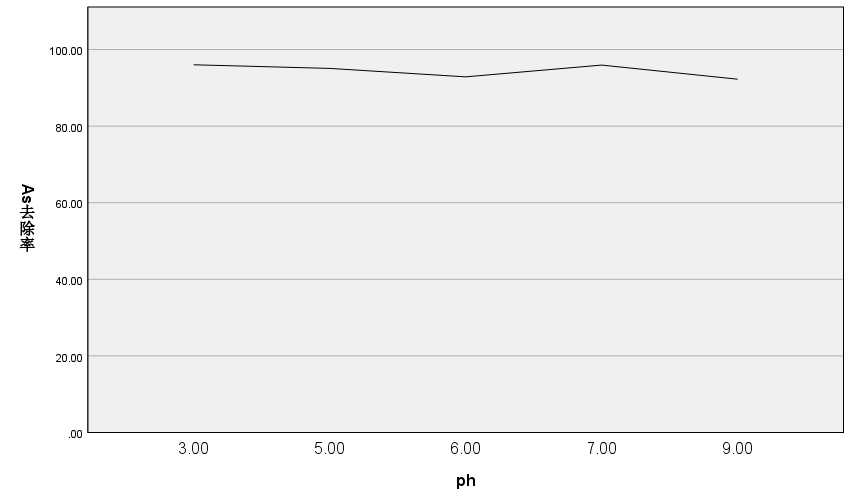
\includegraphics[width=\linewidth]{phAs.png}
			\caption*{pH对As去除率的回归曲线}
			\label{fig:image1}
		\end{minipage}
		\hfill
		\begin{minipage}{0.45\textwidth}
			\centering
			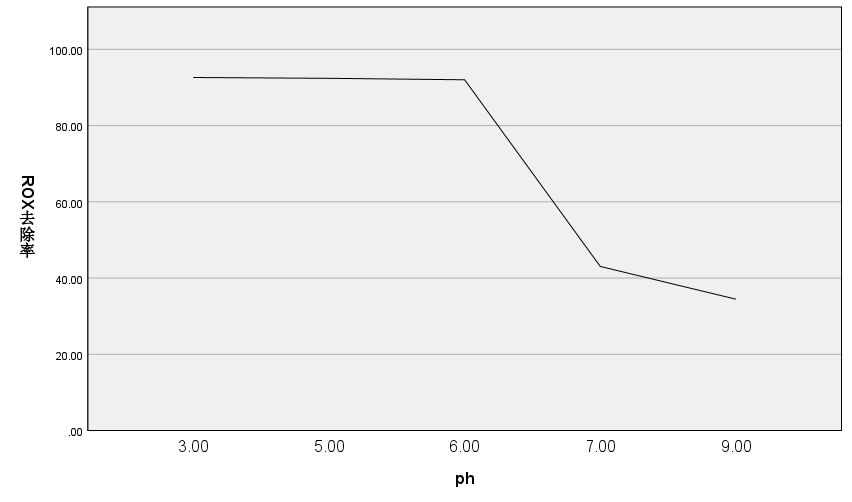
\includegraphics[width=\linewidth]{phROX.png}
			\caption*{pH对ROX去除率的回归曲线}
			\label{fig:image2}
		\end{minipage}
		\caption{pH对去除率的回归曲线}
	\end{figure}
	\begin{figure}[H]
		\centering
		\begin{minipage}{0.45\textwidth}
			\centering
			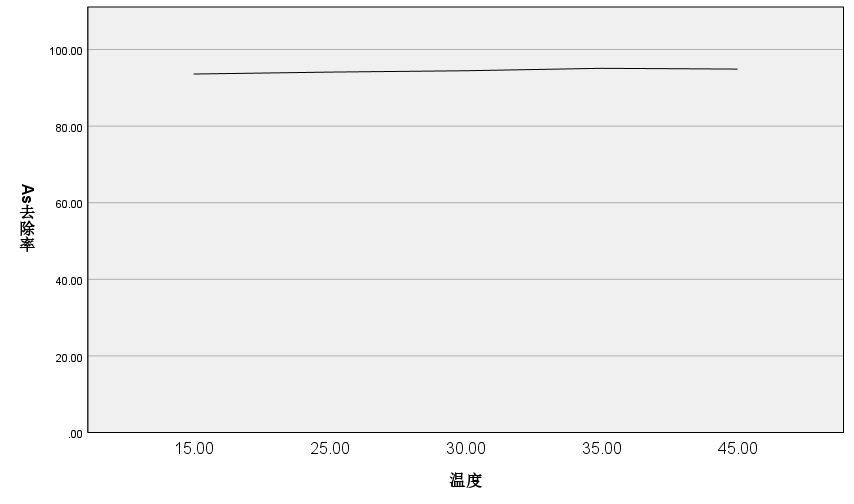
\includegraphics[width=\linewidth]{temAs.png}
			\caption*{温度对As去除率的回归曲线}
			\label{fig:image1}
		\end{minipage}
		\hfill
		\begin{minipage}{0.45\textwidth}
			\centering
			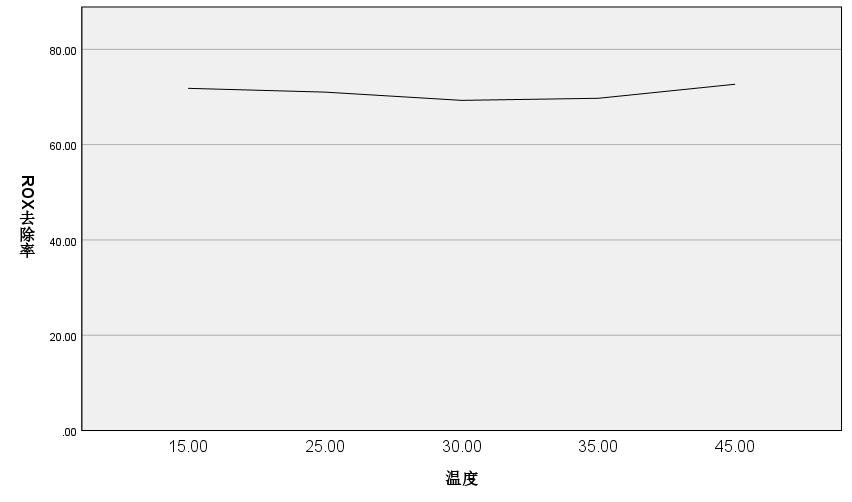
\includegraphics[width=\linewidth]{temROX.png}
			\caption*{温度对ROX去除率的回归曲线}
			\label{fig:image2}
		\end{minipage}
		\caption{温度对去除率的回归曲线}
	\end{figure}
	\begin{figure}[H]
		\centering
		\begin{minipage}{0.45\textwidth}
			\centering
			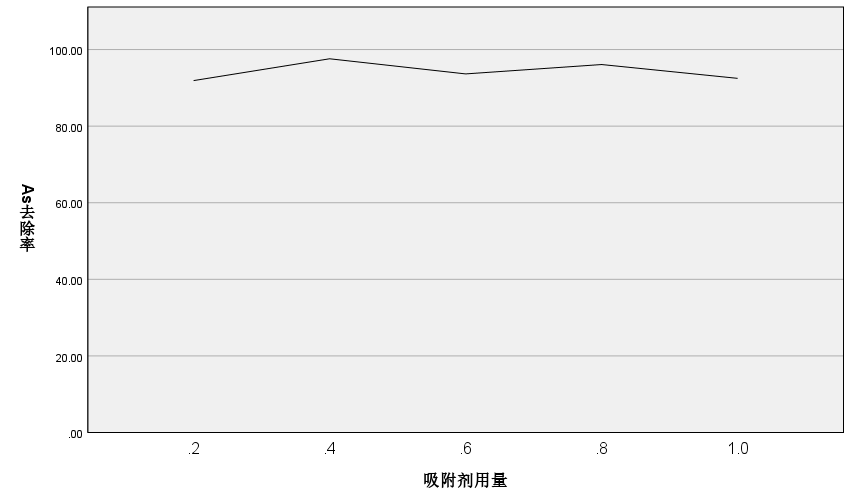
\includegraphics[width=\linewidth]{numAs.png}
			\caption*{吸附剂用量对As去除率的回归曲线}
			\label{fig:image1}
		\end{minipage}
		\hfill
		\begin{minipage}{0.45\textwidth}
			\centering
			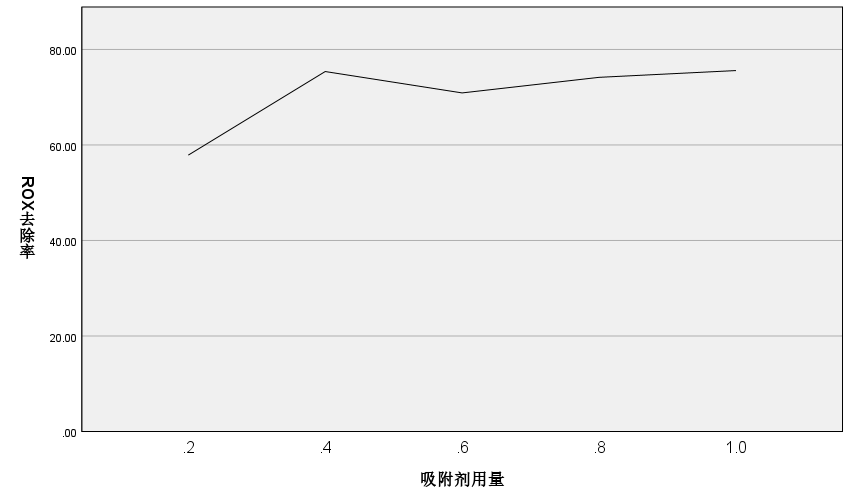
\includegraphics[width=\linewidth]{numROX.png}
			\caption*{吸附剂用量对ROX去除率的回归曲线}
			\label{fig:image2}
		\end{minipage}
		\caption{吸附剂用量对去除率的回归曲线}
	\end{figure}
	
	

	

	
	\subsection{问题二}
	
	\songti\zihao{-4}在问题一的求解中,本文通过建立多元变量模型,初步了解了pH,温度,吸附剂用量对去除率的大致影响趋势,并进行了图像上的展示,
	\songti\zihao{-4}问题二在问题一的基础上对数据进行进一步处理,将数据与弗罗因德利希模型进行拟合,综合测算各变量对于吸收量的影响,并基于梯度提升机方法对各变量进行迭代测试,最终优化出最佳的条件使得总吸附量趋于最大
	\subsubsection{对于吸附模型的建立}
	\songti\zihao{-4}\textbf{弗罗因德利希模型}是描述液相与气相有机物与无机物吸附的经典模型,常用于描述非均匀表面多孔吸附物的吸附能力,本文参考给出的具体情境选择采用该模型进行模拟。\cite{kano2000fractal}
	\songti\zihao{-4}同时由于弗罗因德利希模型是基于科学观测的经验模型,具有一定的局限性,无法反应在较高浓度的吸附现象,也过于依赖实验数据的拟合。
	\subsubsection{目标函数的确定}
	\songti\zihao{-4}本题的优化目标是通过\textbf{弗罗因德利希模型}对于影响其系数的pH,温度,吸附剂用量进行优化,从而得到最高的总吸附量。
	
	这是模型的具体展现
	\begin{equation}
		Q_e = K_f*C_e^{\frac{1}{n}}
		\label{eq:eq1}
	\end{equation}
	
	通过题目给出:
	
	去除率:吸附前后污染物质量浓度差与吸附前污染物质量浓度的比值。即
	\begin{equation}
		R(\%) = \frac{(C_0-C_e)}{C_0}*100
		\label{eq:eq2}
	\end{equation}
	式中 R 是去除率,$C_0$ 是污染物初始质量浓度,$C_e$ 是平衡浓度。
	
	吸附量:单位质量吸附剂所能吸附的最大污染物质量,即
	\begin{equation}
		Q_e = \frac{(C_0-C_e)*V}{m}
		\label{eq:eq3}
	\end{equation}
	式中 $Q_e$ 是吸附量,$C_0$、$C_e$ 同上,V 是溶液体积,m 是吸附剂质量。
	
	可以推出平衡浓度与吸附量之间的关系为:
	
	
	
	
	\begin{equation}
		C_e  =  \frac{Q_e*m}{v}*\frac{1-R}{R}
		\label{eq:eq4}
	\end{equation}
	代入具体数据,可以得出$K_f$的大致范围。进而求得总吸附量的估计值
	为了使总吸附量最大,可以将$K_f$与pH,温度,吸附剂用量关系表示为以下公式:
	
	\begin{equation}
		K_f=f(T,pH,m)
		\label{eq:eq5}
	\end{equation}
	
	对于该公式的拟合,初步实验选择了沿用实验一方法,使用了多元线性回归模型进行建模,结果发现该模型决定系数$R^2$为0.41,这个值相对较低,说明该模型的拟合程度较差,可能最终得到的各变量值误差较大,因此本文决定摒弃该模型,不过该模型仍然展现了一些特点,如较高的吸附剂用量可能有助于提高吸附容量,而较低的pH和温度可能更有利于吸附。
	
	
	通过梯度提升机法,模型的决定系数显著提高到0.85,这表明该方法能够有效地对数据中的复杂关系进行捕捉。
	
	\subsubsection{模型求解}
	对于模型的求解上,为了简化计算在初步建立弗罗因德利希吸附模型时,假定了n=1,减少了模型的复杂度,在初次建模中先从简单的线性模型进行拟合,渐进到较为复杂的机械学习模型,这使得后续的模型选择更易于比较,在算法方面,使用预设的GBM模型,允许自动处理特征间的非线性关系与交互作用,减少了手动设定的麻烦。
	
	对于模型的计算,首先使用推导出的平衡密度与总吸附量公式计算出各条件下平衡浓度,然后使用\textbf{计算$K_f$的Python代码}(见附录A:(1))[\ref{key:1}],得到$K_f$的大概值为16.25。
	
	然后使用公式(5)[\ref{eq:eq5}],通过\textbf{梯度提升法},先对所有的特征进行标准化处理,来消除量纲影响并加快模型收敛速度,使用梯度提升机算法在训练集上训练,调整模型参数如学习率,树的数量和最大树深度等,通过迭代方式训练多个决策树,每颗树都尝试去纠正前一个树留下的错误。\cite{friedman2001greedy}使用\textbf{最优解模型}(见附录A:(3))\pageref{cite:3}可以得到,达到最大总吸附量的最优条件如下:
	
	\begin{table}[H]
		\centering
		\begin{tabular}{ccc}
			\toprule
			pH值 & &3.0 \\
			
		吸附剂用量(m) & & 0.2 \\
			温度 & & 30(摄氏度) \\
			预测总吸附量 & & 约45.29 \\
		
			\bottomrule
		\end{tabular}
		\caption{模型公式所用的符号解释表}
		\label{tab:example}
	\end{table}
	
	\subsection{问题三}
	\subsubsection{中心点重复实验}
	本实验采用中心点重复的方法,用于评估实验的随机误差和模型的精确度。以下是如何在MATLAB中设计并实现中心点重复实验的步骤和示例代码。
	实验设计步骤
	
	\begin{enumerate}
		\item 确定实验因素:本实验中自变量为反应温度、溶液pH和吸附剂用量。
		\item 确定中心点:对于每个因素,确定其在实验设计中的中心点水平。在本实验中,反应温度、溶液pH和吸附剂用量的中心点水平分别为30,3,0.2。
		\item 设置重复次数:本实验中决定在中心点进行5次重复实验。
		\item 收集数据:在中心点水平上重复进行实验,并记录每次的响应值。
		\item  计算响应值的平均值和标准差,以评估实验误差。
		
	\end{enumerate}
	
	\subsubsection{边界探索性实验}
	
	\begin{enumerate}
		\item 实验点设计:\\
		
			\begin{table}[H]
			\centering
			\begin{tabular}{ccc}
				\toprule
				pH值 &3.0 &9.0 \\
				
				吸附剂用量(m) &0.2g/L & 1.0g/L\\
				温度 &15(摄氏度) & 45(摄氏度) \\
				
				
				\bottomrule
			\end{tabular}
			\caption*{}
			\label{tab:example1}
		\end{table}
		
	
		
		\item 实验执行:在上述设计的实验点上进行实验,记录As(V)和 ROX 的总吸附 
		量。
		
		\item 数据分析:比较实验结果与模型预测,检查是否有未被模型捕捉到的新趋势或效应。
		\item 模型更新:如果发现新的趋势,根据实验数据更新模型。
		
		
	\end{enumerate}
	
	通过这样的探索性实验设计,我们可以更好地理解模型的局限性,并可能发现新的科学现象或工艺改进的机会,从而使得所建数学模型更具有普遍性和健壮性。
	
	\subsubsection{敏感性分析实验}
	
	敏感性分析是评估模型中各个参数对输出结果影响程度的一种方法。在环境工程、化学工程或材料科学等领域,了解哪些因素对特定响应(如As(V)和 ROX 的总吸附量)最为敏感,可以帮助研究人员优化实验条件和工艺参数。
	
		\begin{enumerate}
		\item 确定模型和响应:本实验中使用的数学模型为弗罗因德利希模型,此次将要评估的响应变量为As(V)和ROX的总吸附量。
		\item 识别关键参数:基于先前实验或理论认识,识别可能对响应变量(As(V)和ROX的总吸附量)有显著影响的参数。
		\item 设计实验矩阵:创建一个实验设计矩阵,系统地改变关键参数,同时保持其他参数在固定水平。
		\item 数据分析:分析实验结果,评估每个参数的变化对响应变量的影响。
		\item  评估敏感性:确定哪些参数对响应变量最为敏感,可以通过计算每个参数变化时响应变量的变化百分比来评估。
		\item  模型调整:根据敏感性分析的结果,调整模型以更好地反映敏感参数的影响。
	\end{enumerate}
	
	\subsubsection{验证实验}
	
	验证实验是确认模型预测的最优条件是否在实际操作中有效的重要步骤。在通常涉及到在测的最优条件下重复实验,以此可以确保结果的一致性和可靠性,提高实验结果的稳定性。
	
	实验设计步骤
	
	\begin{enumerate}
		\item 模型预测:基于先前实验数据,使用弗罗因德利希模型预测最优条件。
		\item 确定验证条件:从模型预测中得到最优的条件组合。
		\item 设计验证实验:设计一系列实验来验证这些最优条件。
		\item 执行实验:在选定的最优条件下执行实验,收集数据。
		\item  数据分析:分析实验结果,比较模型预测和实验观察。
		\item  评估一致性:评估实验结果与模型预测的一致性。
		\item  报告结果:编写实验报告,包括实验设计、结果和结论
	\end{enumerate}
	
	\subsubsection{环境因素识别实验}
	
	在进行化学实验时,环境因素可能会影响实验结果的准确性和可重复性。通过进行环境因素识别实验,可以最大限度减小环境因素对实验结果的影响,提高实验模型的稳定性与健壮性。
	实验设计步骤
	
	\begin{enumerate}
		\item 环境因素识别:识别所有可能影响实验结果的环境因素,例如湿度、气压、光照强度、空气流动等。
		\item 环境控制:使用湿度控制器、遮光幕布、气流控制系统等设备来维持稳定的实验环境。
		\item 实验材料和试剂的一致性:确保所有实验材料和试剂的批次一致,避免批次差异对实验结果的影响。
		\item 实验设备的校准:
		定期校准实验中使用的仪器设备,如pH计、温度传感器等。
		\item  实验操作的标准化:
		制定详细的实验操作规程,确保每次实验的步骤和条件一致。
		\item  实验监控:
		在实验过程中实时监控环境因素,记录任何可能的变化。
		\item  数据记录:记录所有实验条件和结果,包括环境因素的详细数据。
		\item  实验重复:进行多次重复实验以验证结果的可重复性。
	\end{enumerate}
	
	\section{模型的分析与检验}
	\begin{enumerate}
		\item 计算预测值:
		
		 使用拟合的有梯度提升机优化后的弗伦德利希等温线模型参数($K_F$ 和 $n$)来计算平衡浓度($C_e$)对应的吸附量($Q_e$)的预测值。
		
		\item 计算拟合优度:
		
		 计算残差(实际观测值与模型预测值之间的差异)。
		
		 使用残差来计算总平方和和残差平方和,从而得到决定系数($R^{2}$),用以评估模型解释数据变异性的能力。
		
		 计算平均绝对误差(MAE)和均方误差(MSE)以进一步评估模型的表现。
		\item 绘制残差图:
		
		 绘制另一个图表,显示每个平衡浓度点的残差(实际观测值减去预测值)。
		
		 残差图用来检查是否存在系统误差或特定模式,这可能表明模型对数据的拟合不够好。
		\end{enumerate}
		\begin{figure}[H]
			\centering
			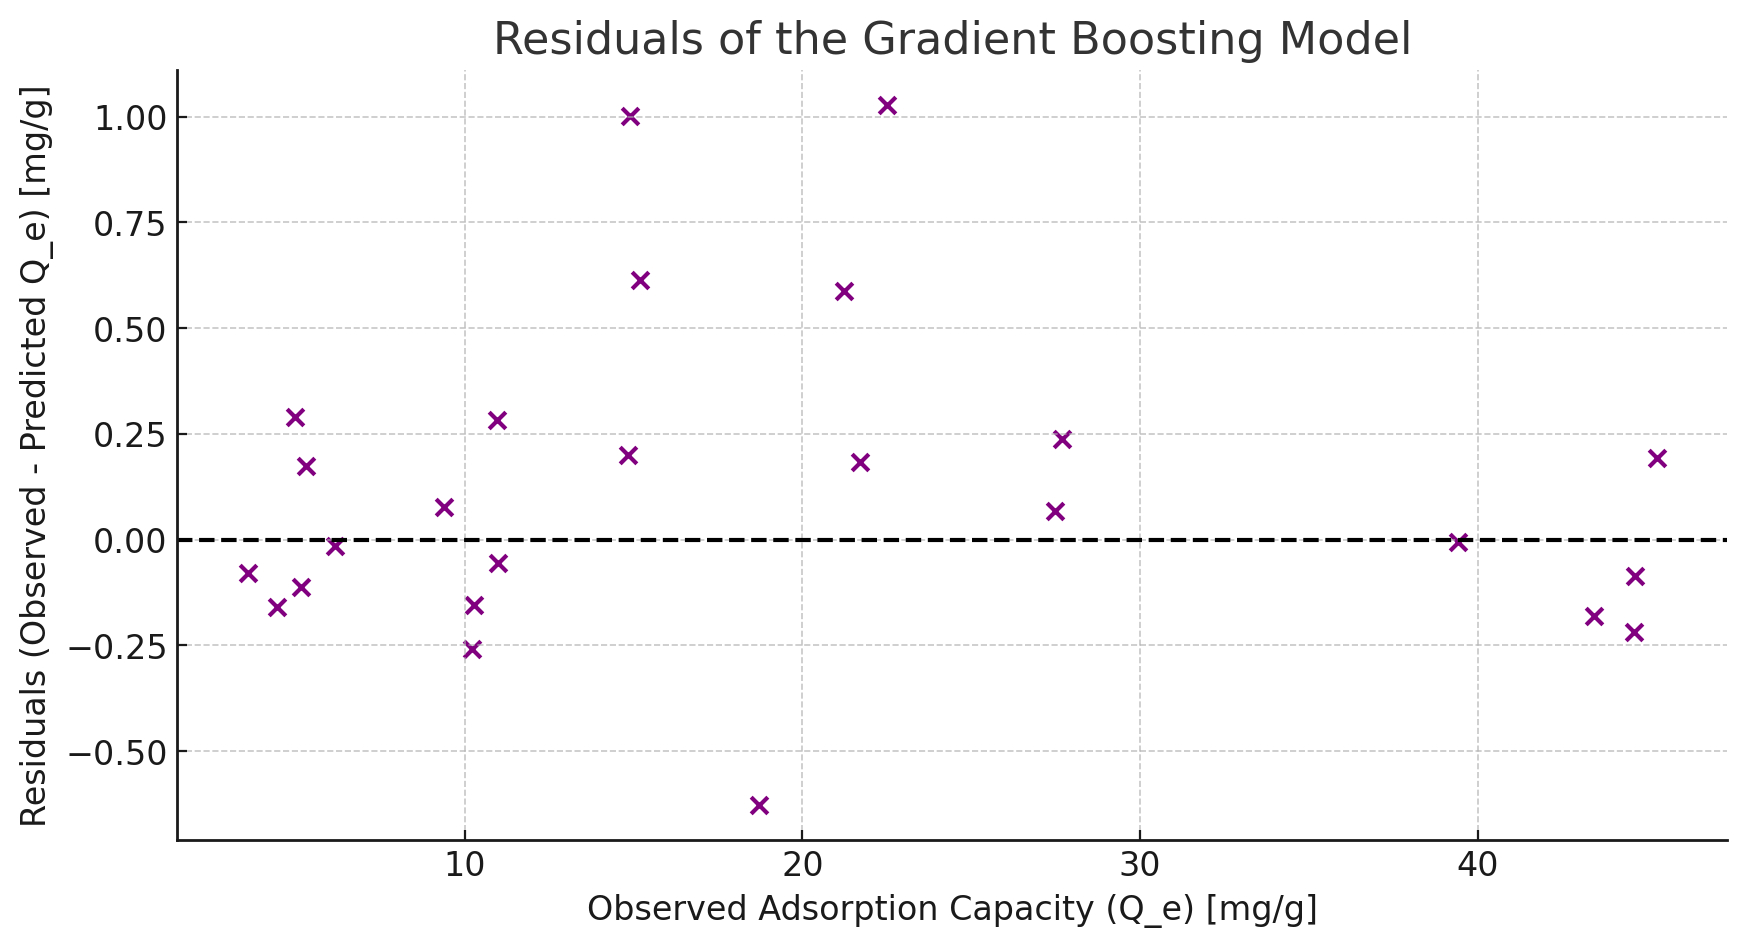
\includegraphics[width=0.65\textwidth]{残差.png}
			\caption{残差图}
			\end{figure}
				
				残差分布在零线周围,大多数残差靠近零,说明模型的预测与实际观测值非常接近。没有明显的系统偏差或模式,表明模型对数据的拟合是适当的。\\
					
		使用优化后的梯度提升机(GBM)模型进行的预测表现非常好,具体表现如下:
		
		均方误差(MSE):0.15 $(mg/g)^2$
		
		决定系数(R²):0.9992
		
		这意味着优化后的GBM模型解释了测试数据中近99.92\%的变异性,显著优于之前使用的弗伦德利希模型。这个高决定系数表明模型非常适合这组数据。
	\section{模型的评价、改进与推广}
	\subsection{问题一:}
	\subsubsection{评价:}
	 问题一所使用的多元线性回归模型可以对数据简单地进行统计,在一定情况下可以准确地满足现实的需要。但是该方法过于简化现实:线性模型可能无法很好地描述复杂的和非线性的现实世界关系。并且易受异常值影响:异常值和杠杆点可以极大地扭曲回归系数和模型的整体拟合。
	\subsubsection{改进建议:}
	可以对数据进行预处理,剔除数据中的异常值。可以对模型进行交叉验证,确保模型在未知数据上表现的稳定;可以分析残差图检查模型,进一步调整模型和数据。
	
	\subsection{问题二:}
	\subsubsection{评价:}
	改进使用梯度提升机(GBM)模型对吸附数据进行拟合带来了显著的提升,特别是在预测准确性和模型解释性方面。以下是对该模型改进的具体评价:
	
	1. 预测准确性提高:
	 GBM模型的均方误差(MSE)非常低(0.15),决定系数($R^2$)接近1(0.9992),这表明模型能够非常精确地预测吸附量。这一性能指标远超前面使用的弗伦德利希模型。
	
	2. 无明显的残差偏差:
	 残差图显示残差主要集中在零附近,没有显示出任何系统性偏差或特定的模式,这表明模型预测与实际观测值之间误差较小,模型拟合效果良好。
	
	3. 重要的特征洞察:
	 特征重要性分析揭示了吸附剂用量和平衡浓度是影响吸附量最关键的因素。这种洞察可以帮助优化实验设计和操作条件,进一步提高吸附过程的效率和效果。
	
	4. 模型的灵活性和扩展性:
	 GBM能够处理非线性关系和复杂的交互作用,这使得它适用于各种复杂的实际应用场景。此外,GBM模型的参数(如树的数量、学习率和最大深度)可以进一步调整优化,以适应不同的数据集和特定需求。\cite{friedman2001greedy}
	
	 \subsubsection{改进建议:}
	
	尽管GBM模型表现出色,仍有一些方面可以进一步探索以优化模型:
	
	1.参数调优:可以使用网格搜索(Grid Search)或随机搜索(Random Search)来优化GBM的超参数,寻找最佳的学习率、树的数量和深度等,以实现更优的性能。\cite{jain2016complete}
	
	2.交叉验证:应用交叉验证方法可以更全面地评估模型的稳定性和泛化能力,确保模型在不同的数据子集上都能维持高性能。\cite{xue2011极限学习机的快速留一交叉验证算法}
	
	3.模型集成:考虑将GBM与其他类型的机器学习模型(如随机森林、支持向量机等)进行集成,以进一步提高预测的准确性和鲁棒性。
	
	
	
	\section{参考文献}
	\bibliographystyle{plain}
	\bibliography{references}
	\newpage
	\section{附录}
	\subsection{附录A:代码部分}
 \centering\textbf{(1)计算$K_f$的Python代码:}
 \label{key:1}
 \lstset{language=Python}
 \lstset{breaklines}%自动将长的代码行换行排版
 \begin{lstlisting}
 	import pandas as pd
 	
 	path = "E:/onedrive/Desktop/数模/模型变量.xlsx"
 	data = pd.read_excel(path)
 	# 显示数据
 	data.head()
 	from scipy.optimize import curve_fit
 	import numpy as np
 	#定义模型
 	def freund(C_e, K_F, n):
 	return K_F * C_e ** (1/n)
 	#将吸附量与平衡浓度导入
 	C_e = data['C_e']
 	Q_e = data['Q_e']
 	# 拟合
 	initial_guess = [1, 1]  # K_F 和 n 的初始猜测值
 	params, covariance = curve_fit(freund, C_e, Q_e, p0=initial_guess)
 	# 提取拟合参数
 	K_F, n = params
 	K_F, n
 	# 计算参数
 	data['predicted_Q_e'] = freund(data['C_e'], K_F, n)
 	# 找到实际 Q_e 最大的条件
 	max_Qe_conditions = data.loc[data['Q_e'].idxmax(), ['ph', '吸附剂用量', '温度', 'Q_e']]
 	
 	max_Qe_conditions
 	
 \end{lstlisting}
 \newpage
  \centering\textbf{(2)第一次线性拟合的Python代码:}\label{cite:2}
 \lstset{language=Python}
 \lstset{breaklines}%自动将长的代码行换行排版
 \begin{lstlisting}
 import pandas as pd
 from sklearn.preprocessing import StandardScaler
 from sklearn.model_selection import train_test_split
 from sklearn.linear_model import LinearRegression
 from sklearn.metrics import r2_score
 import pandas as pd
 
 path = "E:/onedrive/Desktop/数模/模型变量.xlsx"
 new_data = pd.read_excel(path)
 def K_F(row):
 n_F = 1  # 假设 n_F = 1 
 K_F = row['Q_e'] / (row['C_e'] ** (1 / n_F))  # 使用简化的方程计算 K_F
 return K_F
 # 函数计算集中每行的 K_F
 new_data['K_F'] = new_data.apply(K_F, axis=1)
 #对变量建模
 feature = new_data[['ph', '吸附剂用量', '温度']]
 target_K_F = new_data['K_F']
 # 标准化新模型
 scal = StandardScaler()
 features_scaled_K_F = scal.fit_transform(feature)
 
 # 拆分数据
 X_train_K_F, X_test_K_F, y_train_K_F, y_test_K_F = train_test_split(features_scaled_K_F, target_K_F, test_size=0.2, random_state=42)
 
 # 创建并训练 K_F 的线性回归模型
 model_K_F = LinearRegression()
 model_K_F.fit(X_train_K_F, y_train_K_F)
 
 # 预测并评估 K_F 模型
 prediction = model_K_F.predict(X_test_K_F)
 r2 = r2_score(y_test_K_F, prediction)
 
 # 显示 K_F 模型系数和 R² 
 model_coeffi = model_K_F.coef_
 intercep = model_K_F.intercept_
 print("(R^2)分数:", r2)
 print("模型系数:", model_coeffi)
 print("截距:", intercep)
 
 \end{lstlisting}
  \label{cite:3}

 
\centering\textbf{(3)最大吸附量下pH、温度与吸附剂用量数据最优解模型的Python代码:}

 \lstset{language=Python}
 \lstset{breaklines}%自动将长的代码行换行排版

 \begin{lstlisting}
 	import pandas as pd
 	
 	data_path = "E:/onedrive/Desktop/数模/总数据.xlsx"
 	data = pd.read_excel(data_path)
 	
 	data.head()
 	
 	from sklearn.ensemble import GradientBoostingRegressor
 	from sklearn.model_selection import train_test_split
 	
 	# 添加一个新列用于总吸附量
 	data['总吸附量'] = data['ROX吸附量'] + data['As吸附量']
 	
 	# 准备特征矩阵和目标向量
 	X = data[['ph', '吸附剂用量', '温度']]
 	y = data['总吸附量']
 	
 	# 将数据集拆分为训练集和测试集
 	X_train, X_test, y_train, y_test = train_test_split(X, y, test_size=0.2, random_state=42)
 	
 	# 初始化梯度提升回归器
 	model = GradientBoostingRegressor(n_estimators=100, learning_rate=0.1, max_depth=3, random_state=42)
 	
 	# 拟合模型
 	model.fit(X_train, y_train)
 	
 	# 在整个数据集上进行预测以找到最大吸附量
 	data['预测总吸附量'] = model.predict(X)
 	
 	# 找到给出最大总吸附量的条件
 	optimal_conditions = data.loc[data['预测总吸附量'].idxmax()]
 	
 	optimal_conditions
 \end{lstlisting} 
 
 \centering\textbf{(4)数据预处理的Python代码:}

 \lstset{language=Python}
 \lstset{breaklines}%自动将长的代码行换行排版
 
 \begin{lstlisting}
 	import pandas as pd
 	
 	# 加载数据
 	data_path = "E:/onedrive/Desktop/数模/总数据.xlsx"
 	data = pd.read_excel(data_path)
 	# 定义函数来识别和删除异常值
 	def remove_outliers(df):
 	for column in df.select_dtypes(include=['float64', 'int64']):
 	Q1 = df[column].quantile(0.25)
 	Q3 = df[column].quantile(0.75)
 	IQR = Q3 - Q1
 	lower_bound = Q1 - 1.5 * IQR
 	upper_bound = Q3 + 1.5 * IQR
 	
 	# 过滤异常值
 	outliers = df[(df[column] < lower_bound) | (df[column] > upper_bound)]
 	df = df.drop(outliers.index)  # 删除异常值
 	return df
 	
 	
 	# 应用函数
 	cleaned_data = remove_outliers(data)
 	
 	# 保存清洗后的数据
 	cleaned_data.to_excel("清洗后的数据.xlsx", index=False)
 	
 	# 显示部分清洗后的数据
 	print(cleaned_data.head())
 \end{lstlisting} 
 
 \centering\textbf{(5)中心点重复试验的MATLAB代码:}
 \lstset{language=MATLAB}
 \lstset{breaklines}%自动将长的代码行换行排版
 \begin{lstlisting}
 	% 设定自变量的中心点水平
 	temperature = 30; % 反应温度
 	pH = 3;           % 溶液pH
 	adsorbent_amount = 0.2; % 吸附剂用量
 	
 	% 设定重复次数
 	repetitions = 5;
 	
 	% 初始化响应值数组
 	responses = zeros(repetitions, 1);
 	
 	% 进行重复实验
 	for i = 1:repetitions
 	% 这里假设 experimental_function 是一个根据自变量返回响应值的函数
 	response = experimental_function(temperature, pH, adsorbent_amount);
 	responses(i) = response;
 	end
 	
 	% 计算平均值和标准差
 	mean_response = mean(responses);
 	std_dev = std(responses);
 	
 	% 打印结果
 	fprintf('中心点重复实验的平均响应值:%f\n', mean_response);
 	fprintf('中心点重复实验的标准差:%f\n', std_dev);
 	
 	% 评估实验误差
 	if std_dev < 1 % 假设1是可接受的误差阈值
 	disp('实验误差较小,结果稳定。');
 	else
 	disp('实验误差较大,需要进一步调查原因。');
 	end
 	
 	% 假设的实验函数,这里使用随机数模拟响应值
 	function response = experimental_function(temperature, pH, adsorbent_amount)
 	% 模拟As(V)和ROX的去除率
 	response = normrnd(100, 5); % 正态分布的随机数,均值为100,标准差为5
 	end
 \end{lstlisting}
 
 \centering\textbf{(6)边界探索性试验的MATLAB代码:}
 \lstset{language=MATLAB}
 \lstset{breaklines}%自动将长的代码行换行排版
 \begin{lstlisting}
%模拟实验响应函数:simulate_experiment函数用于模拟在给定条件下的实验响应。这里我们使用了一个简单的线性模型,但您可以根据实际情况替换为更复杂的模型。
%边界条件:定义了温度、pH和吸附剂量的最小值和最大值。
%探索性实验设计:创建了一个矩阵exploration_points,包含了我们想要探索的实验点。这些点可能位于模型预测的边界或未探索区域。
%进行探索性实验:循环遍历每个探索点,调用simulate_experiment函数来模拟实验,并收集响应。打印结果:打印每个探索点的响应,以供进一步分析。

 % 假设的实验响应函数,模拟实验结果
 function response = simulate_experiment(temperature, pH, adsorbent_amount)
 % 这里使用一个简单的数学模型来模拟响应
 response = 100 + 5 * temperature - 2 * pH + 10 * adsorbent_amount;
 end
 
 % 边界条件
 min_temperature = 15;   % 最低温度
 max_temperature = 45;   % 最高温度
 min_pH = 3;             % 最低pH
 max_pH = 9;            % 最高pH
 min_adsorbent_amount = 0.2; % 最小吸附剂量
 max_adsorbent_amount = 1.0; % 最大吸附剂量
 
 % 探索性实验设计
 exploration_points = [
 min_temperature, max_pH, min_adsorbent_amount; % 边界条件1
 max_temperature, min_pH, max_adsorbent_amount; % 边界条件2
 (min_temperature + max_temperature) / 2, (min_pH + max_pH) / 2, min_adsorbent_amount; % 中心点
 (min_temperature + max_temperature) / 2, (min_pH + max_pH) / 2, max_adsorbent_amount; % 中心点与最高剂量
 ];
 
 % 进行探索性实验
 responses = zeros(size(exploration_points, 1), 1);
 
 for i = 1:size(exploration_points, 1)
 [temperature, pH, adsorbent_amount] = deal(exploration_points(i, :));
 responses(i) = simulate_experiment(temperature, pH, adsorbent_amount);
 end
 % 打印结果
 for i = 1:length(responses)
 fprintf('实验点%d的响应:%f\n', i, responses(i));
 End
 
 
 
 \end{lstlisting}
 
 \centering\textbf{(7)敏感性分析实验的MATLAB代码:}
 \lstset{language=MATLAB}
 \lstset{breaklines}%自动将长的代码行换行排版
 \begin{lstlisting}
 	%experimental_response函数是一个模拟函数,用于根据输入参数计算响应值。
 	%定义了关键参数的范围,这里以温度、pH和吸附剂量为例。
 	%创建了一个实验设计矩阵experiment_matrix,用于系统地改变每个参数。
 	%执行实验并收集数据,存储在responses数组中。
 	%对收集到的数据进行简单分析,这里计算了每个参数在不同水平下的平均响应,并打印出来。
 	
 	% 假设的实验响应函数,模拟实验结果
 	function response = experimental_response(temperature, pH, adsorbent_amount)
 	% 模拟As(V)和ROX的去除率
 	% 这里使用一个简单的模型,您可以根据实际情况替换为更复杂的模型
 	response = 100 - 2 * temperature + 0.5 * pH - 5 * adsorbent_amount;
 	end
 	
 	% 关键参数的范围
 	temperatures = 15:10:45; % 温度范围
 	pH_values = 3:2:9;     % pH范围
 	adsorbent_amounts = [0.2,0.4,0.6,0.8,1.0]; % 吸附剂量
 	
 	% 其他参数固定水平
 	fixed_temperature = 30; % 固定温度
 	fixed_pH = 3;            % 固定pH
 	
 	% 敏感性分析实验设计
 	experiment_matrix = array2table(...
 	
 	[{temperatures; fixed_temperature*ones(1, length(adsorbent_amounts))}, ...
 	{fixed_pH*ones(1, length(temperatures)); pH_values; fixed_pH*ones(1, length(adsorbent_amounts))}, ...
 	{adsorbent_amounts; adsorbent_amounts; fixed_temperature*ones(1, length(pH_values))}],...
 	
 	'VariableNames', {'Parameter', 'Level'});
 	
 	% 执行实验并收集数据
 	responses = zeros(size(experiment_matrix));
 	
 	for i = 1:height(experiment_matrix)
 	param = experiment_matrix{i, :};
 	responses(i) = experimental_response(param{1}, param{2}, param{3});
 	end
 	
 	% 数据分析和敏感性评估
 	% 这里简单地打印每个参数在不同水平下的平均响应
 	mean_responses = mean(responses, 2);
 	disp(mean_responses);
 	
 \end{lstlisting}
 
 \centering\textbf{(8)验证试验的MATLAB代码:}
 \lstset{language=MATLAB}
 \lstset{breaklines}%自动将长的代码行换行排版
 \begin{lstlisting}
 	%optimal_temperature, optimal_pH, optimal_adsorbent_amount是模型预测的最优条件。
 	%设定了重复次数repetitions,以确保验证实验的统计可靠性。
 	%simulate_experiment函数是一个模拟实验响应的函数,这里使用正态分布随机数模拟响应值。
 	%循环执行验证实验,并收集响应值。
 	%计算响应值的平均值和标准差,以评估实验的一致性。
 	%根据标准差的值评估验证实验结果的一致性,并打印相应的消息。
 	
 	% 假设的最优条件,这些条件是模型预测的结果
 	optimal_temperature = 30;   % 最佳反应温度
 	optimal_pH =3;             % 最佳溶液pH
 	optimal_adsorbent_amount = 0.2; % 最佳吸附剂用量
 	
 	% 设定重复次数
 	repetitions = 5;
 	
 	% 初始化响应值数组
 	responses = zeros(repetitions, 1);
 	
 	% 模拟实验响应函数
 	function response = simulate_experiment(temperature, pH, adsorbent_amount)
 	% 这里使用一个简单的模型来模拟响应
 	response = normrnd(100, 5); % 正态分布的随机数,均值为100,标准差为5
 	end
 	
 	% 执行验证实验
 	for i = 1:repetitions
 	response = simulate_experiment(optimal_temperature, optimal_pH, optimal_adsorbent_amount);
 	responses(i) = response;
 	end
 	
 	% 计算平均值和标准差
 	mean_response = mean(responses);
 	std_dev = std(responses);
 	
 	% 打印结果
 	fprintf('验证实验的平均响应值: %f\n', mean_response);
 	fprintf('验证实验的标准差: %f\n', std_dev);
 	
 	% 评估结果
 	if std_dev < 2 % 假设2是可接受的误差阈值
 	disp('验证实验结果一致,模型预测可靠。');
 	else
 	disp('验证实验结果不一致,需要进一步研究。');
 	End
 	
 	
 \end{lstlisting}
 \newpage
 \centering\textbf{(9)As吸附率回归方程的SPSS交互命令:}
 \begin{verbatim}
 	REGRESSION
 	/MISSING LISTWISE
 	/STATISTICS COEFF OUTS R ANOVA
 	/CRITERIA=PIN(.05) POUT(.10)
 	/NOORIGIN
 	/DEPENDENT As吸附率
 	/METHOD=ENTER ph 温度 吸附剂用量.
 \end{verbatim}
 
 
 \centering\textbf{(10)ROX吸附率回归方程的SPSS交互命令:}
 \begin{verbatim}
 	REGRESSION
 	/MISSING LISTWISE
 	/STATISTICS COEFF OUTS R ANOVA
 	/CRITERIA=PIN(.05) POUT(.10)
 	/NOORIGIN
 	/DEPENDENT ROX吸附率
 	/METHOD=ENTER ph 温度 吸附剂用量.
 \end{verbatim}
\end{document}


